
\subsubsection{Theorie (O.S.)}
Im Leichtbau ist es wichtig geeignete Konstruktionen zu entwerfen, um Eigenschaften der Werkstoffe ideal nutzen zu können. Das Gesamtbauteil ist dann meist so kompliziert, dass sich die für das Bauteil zu lösenden Differenzialgleichungen, wie zum Beispiel die der Elastostatik, keine geschlossenen Lösungen finden lassen. Das Ziel ist es nun durch Annahmen und Vereinfachungen ein sinnvolles und lösbares Ingenieursmodell zu finden. Alternativ könnten auch Lösungen mittels numerischer Methoden ermittelt werde, hierzu mehr in Kapitel \ref{FEM}.

\paragraph{Zylindrische, dünnwandige Profile}~\\
Häufig werden zylindrische, dünnwandige Profil genutzt, da sie bei vergleichsweiser niedriger Masse noch immer gut Werte bei zum Beispiel der Biegesteifigkeit liefern. Sie kennzeichnen sich dadurch aus, dass deutlich höhere Ausmaße in x-Richtung haben, als in jede andere (zylindrisch). Eine Laufvariable $s$ verläuft in der y-z-Ebene durch die Mitte der Profildicke $t(s)$. Die Dicke ist nicht zwangsläufig über $s$ konstant, muss aber deutlich kleiner als alle anderen Abmessungen sein (dünnwandig) \cite{item15}. Man kann vereinfacht annehmen
\begin{equation}
	\iint dA=\int t(s)ds.
\end{equation} 
Der Querschnitt muss in x-Richtung konstant sein und auch bei Belastung seine Gestalt beibehalten. Der Schubfluss im Profil ist als
\begin{equation}\label{tau}
	q=\tau t(s)
\end{equation}
und der Normalkraftfluss als
\begin{equation}
	n_x=\sigma_x t(s)
\end{equation}
definiert. Für diese Kraftflüsse gilt das hydrodynamische Analogon. Das heißt mit einer Änderung der Dicke muss der Kraftfluss antiproportional ab- bzw. zunehmen, damit das Kräftegleichgewicht erfüllt bleibt. Für Knotenpunkte muss auch gelten, dass der Betrag der Kraftflüsse in den Knoten hinein denen aus ihm heraus gleichen. Des Weiteren lässt sich noch zwischen offenen und geschlossenen Profilen unterscheiden, wobei es sich bei zweiterem um Ein- oder Mehrzeller handeln kann.\cite{item15}

\paragraph{Koordinatensysteme}~\\
Bei den Berechnungen kann viel Arbeit gespart werden, indem das Koordinatensystem mit Ursprung und Achsenausrichtung klug gewählt wird. Das allgemeine Koordinatensystem, das unabhängig vom betrachteten Profil ist, bietet hierbei die wenigstem um nicht zu sagen keine Vorteile. Verschiebt man seinen Ursprung in den Schwerpunkt erhält man das Schwerpunkt-Koordinatensystem. Es wird mit einem Querstrich über den Koordinaten gekennzeichnet ($\bar{x},\bar{y},\bar{z}$). Es ist sinnvoll aus dieser Perspektive den Schubfluss zu betrachten.
\begin{figure}[h]
	\centering
	\includegraphics[width=1\textwidth]{Bilder/schubfluss-infinit}
	\caption{Infinitesimales Profilelement aus \cite{item15}}
	\label{schubfluss-infinit}
\end{figure}
Aus dem Kräftegleichgewicht in $x$- und $s$-Richtung an einem infinitesimalen Volumen des dünnwandigen Profils ergibt sich der Zusammenhang zwischen den Kraftflüssen zu
\begin{equation}
	\frac{\partial n_x}{\partial x} + \frac{\partial q}{\partial s} = 0
\end{equation}
\begin{equation}\label{n_s}
\frac{\partial n_s}{\partial s} + \frac{\partial q}{\partial x} = 0
\end{equation}
Da jedoch eine Krümmung in $s$-Richtung vorliegen kann, zeigt die Resultierende des Normalkraftflusses $n_s$ aus der Ebene heraus. Da bei dünnen Scheibenelementen ein ebener Spannungszustand herrscht, darf dies nicht sein. Daraus folgt, dass beide Terme in Gleichung \ref{n_s} gleich null sein müssen. Der Schubfluss ist also in $x$-Richtung konstant und lässt sich somit zu
\begin{equation}
	q(s)=-\int\frac{\partial n_x(x,s)}{\partial x}ds+q_0.
\end{equation}
integrieren. Wird nun der Normalkraftfluss in Abhängigkeit von der Querkraft $Q$ gesetzt, ergibt sich die $Q$-$SI$nen-Formel nach \cite{item15}:
\begin{equation}\label{qs}
	q(s)=-(Q_{\bar{z}}\frac{S_{\bar{y}}(s)I_{\bar{z}}-S_{\bar{z}}(s)I_{\bar{yz}}}{I_{\bar{y}}I_{\bar{z}}-I_{\bar{yz}}^2}+Q_{\bar{y}}\frac{S_{\bar{z}}(s)I_{\bar{y}}-S_{\bar{y}}(s)I_{\bar{yz}}}{I_{\bar{z}}I_{\bar{y}}-I_{\bar{yz}}^2})+q_0
\end{equation}
Mit den Flächenträgheitsmomenten $I$ (siehe Gleichungen \ref{FT1}-\ref{FT3}). Spätestens hier zeigt sich, dass für dieses Modell das Superpositionsprinzip anwendbar ist und man die Kräfte $Q_y$ und $Q_z$ getrennt betrachten kann.
Hier lässt sich direkt erkennen, wie diese Formel durch die Wahl eines besseren Koordinatensystems vereinfacht werden kann. Für das Hauptachsen-Koordinatensystem bleibt der Schwerpunkt weiterhin der Ursprung, jedoch werden die Achsen so um die x-Achse gedreht, dass die Deviationsmomente $I_{yz}$ verschwinden. Es wird mit einem Dach über den Koordinaten gekennzeichnet ($\hat{x},\hat{y},\hat{z}$). Die Integrationskonstante
\begin{equation}
	q_{0} = q_{0b}+q_{0T}
\end{equation}
ist nur bei geschlossenen Profilen ungleich null. Sie sich aus einem Teil, der aus der Biegung entsteht $q_{0b}$ und einem aus der Torsion $q_{0T}$ zusammen. Es gibt einen Punkt in der y-z-Ebene für jedes Profil, wo eine angreifende Kraft keine Torsion verursacht. Dieser Punkt ist von hoher Bedeutung und wir Schubmittelpunkt genannt.
\subsubsection{Idealisierung(H.G.)}
Für die Berechnung des Schubmittelpunkts wird das Flügelprofil als vereinfachter Mehrzeller angenommen.
Dabei wird der Ursprung des Koordinatensystems am unteren rechten Rand gesetzt. Das Modell wird in 10 Teilstrecken $s_{i}$ aufgeteilt. Die Dicke $t$ wird über die Schale konstant angenommen. Der Schaum wird in allen Abschnitten der Schale und im Holm vernachlässigt, da seine Hauptaufgabe der Beulsteifigkeit gilt und er bei der Schubaufnahme im Vergleich zum Laminat nur eine unbedeutende Rolle spielt. Der Steg ist in 2 Abschnitte unterteilt. Für die maximale Belastung und somit für die Auslegung relevant ist nur der Teil mit dem dünneren Gewebe, sodass hier für die Dicke des Stegs $t_{1}=0,314\mathrm{mm}$ angenommen wird. Für die Gurte gilt, dass alle Fasern parallel in x-Richtung ausgerichtet sind. Sie werden in dieser Rechnung ignoriert, da sie folglich im Gegensatz zum $\pm45^\circ$-Gewebe vernachlässigbare Schubkräfte aufnehmen können (D = $t$). Außerdem würde ein über die Dicke variabler Schubmodul die Rechnung unnötig verkomplizieren, da die uns bekannten Methoden zur Schubflussberechnung nur für homogene Werkstoffe gültig sind \cite{item15}.

Diese Annahmen bezüglich des Schaums und der Gurte sind unproblematisch, da sie so getroffen wurden, dass der Flügel sogar noch höheren Belastungen als errechnet standhalten könnte. Als einziges ist zu betrachten, dass durch das Wegfallen des Schaums in der Schale die GFK-Schichten des Sandwichs aufeinander fallen und ihre Position somit um wenige Millimeter ungenau ist. Da die genau errechnete Dicke auf eine Lagenschicht aufgerundet werden muss, ist dies vermutlich kompensierbar, sollte jedoch im Hinterkopf behalten werden.

Abbildung \ref{Fluegel1} zeigt, dass der Profil durch 4 geraden Strecken und einen viertel Kreis modelliert wurde. Die Längen der einzelnen Teilabschnitte lassen sich im Anhang der Abbildung \ref{fig:LaengenS} entnehmen.
\begin{figure}[h]
 \centering
 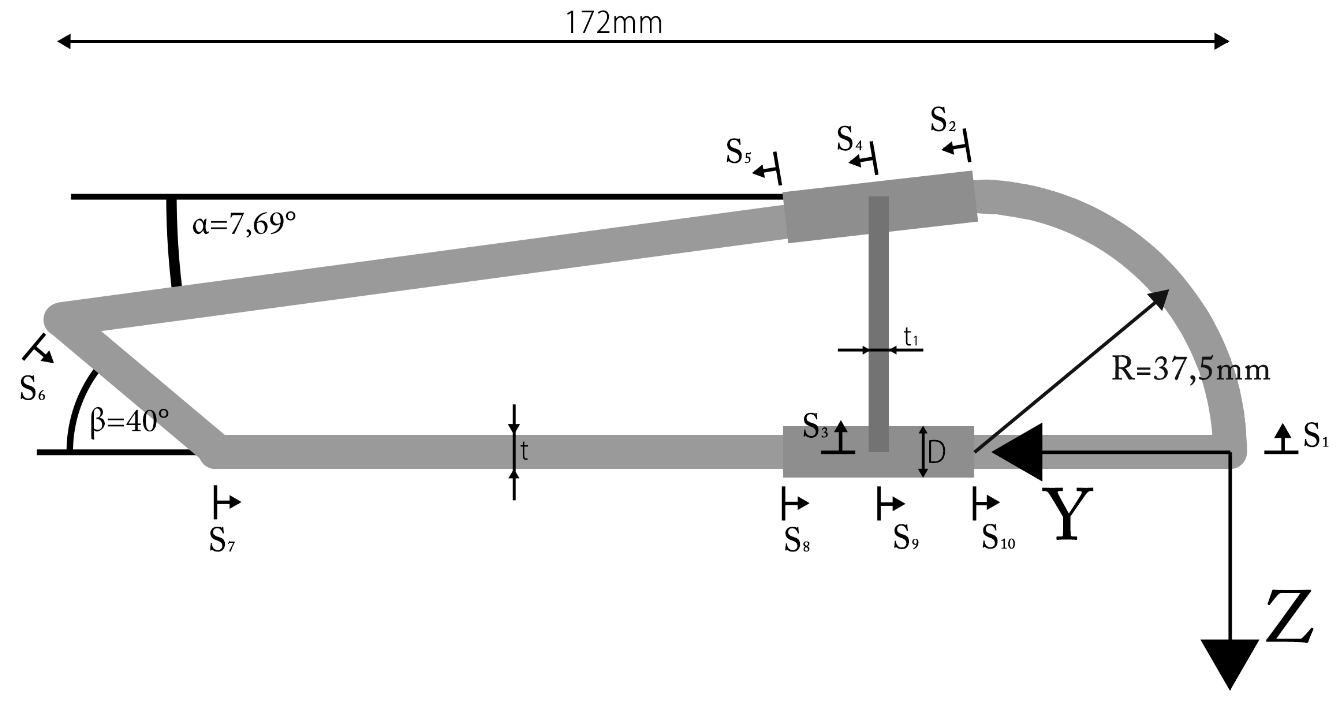
\includegraphics[width=1\textwidth]{Bilder/Model1}
 \caption{vereinfachtes Model}
 \label{Fluegel1}
\end{figure}
\subsubsection{Schwerpunktkoordinaten(H.G.)}\label{SP-Koord}
Zunächst wird von einer Dicke $t=0,2\mathrm{mm}$ ausgegangen und die statischen Momente in den einzelnen Teilstücken berechnet.
\begin{equation}\label{SM1}
	S_{z}=\int_{A}^{}y \mathrm{d}A =t\int_{s}^{}y \mathrm{d}s
\end{equation}
\begin{equation}\label{SM2}
	S_{y}=\int_{A}^{}z \mathrm{d}A =t\int_{s}^{}z \mathrm{d}s 
\end{equation}
Damit ergeben sich für die statischen Momente in $\mathrm{mm}^3$:

\begin{center}
\begin{tabular}[h]{l|c|c}
	
Bauteilabschnitt&$S_{y}/\mathrm{mm}^3$&$S_{z}/\mathrm{mm}^3$\\
\hline
1& -281,25&160,54\\
2&-120,382&124,42\\
3&-220,78&605,24\\
4&-97,13&163,27\\
5&-571,91&2555,63\\
6&-58,13&965,14\\
7&0&1789,88\\
8&0&163,80\\
9&0&124,60\\
10&0&140,63\\
\end{tabular}
\end{center}

\noindent Nun kann aus den statischen Momenten der Schwerpunkt bestimmt werden, indem das Statische Moment über alle Flächen zusammenaddiert wird:
\begin{equation}
	y_{0}=\frac{\int_{s}{}t(s)y\mathrm{d}s}{\int_{s}{}t(s)\mathrm{d}s}=\frac{S_{z}}{A}
\end{equation}
\begin{equation}
	z_{0}=\frac{\int_{s}{}t(s)z\mathrm{d}s}{\int_{s}{}t(s)\mathrm{d}s}=\frac{S_{y}}{A}
\end{equation}
Mit einer Dicke von $t=0,2\mathrm{mm}$ ergeben sich Lagen der Schwerpunktkoordinaten zu:
$$
	y_{0}=78,53\mathrm{mm}
$$
$$
	z_{0}=-15,39\mathrm{mm}
$$

Damit können nun mit
\begin{equation}
	S_{\bar{y}}=S_y-z_0A
\end{equation} 
\begin{equation}
S_{\bar{z}}=S_z-y_0A
\end{equation} 
die Verläufe der statischen Momente in Bezug auf den Schwerpunkt ermittelt werden, wobei die Endwerte der vorherigen Verläufe nach dem hydrodynamischen Analogon den Anfangswert $s_0$ des folgenden Bereichs bestimmen. Dabei ergeben sich folgende Endwerte nach \cite{TMk} in $\mathrm{mm}^3$:
\begin{center}
\begin{tabular}[h]{l|c|c}
Bauteilabschnitt&$S_{\bar{y}}/\mathrm{mm}^3$&$S_{\bar{z}}/\mathrm{mm}^3$\\
\hline
1&-99,91&-764,60\\
2&-159,18&-860,06\\
3&-39,53&-319,43\\
4&-252,75&-1236,10\\
5&-493,03&-372,27\\
6&-458,59&120,60\\
7&-201,65&599,69\\
8&-158,55&543,61\\
9&-155,45&448,34\\
10&0&0\\
\end{tabular}
\end{center}
Für ein offenes Profil muss gelten, dass an den freien Rändern der Schubfluss $ 0 $ ist, was automatisch dadurch erfüllt ist, dass beide statischen Momente ungefähr null sind. Das Profil wird in diesem Fall an den Stellen 1 und 3 geschnitten.


Nun werden die Flächenträgheitsmomente 
\begin{equation}\label{FT1}
	I_{y} = \int_{A}^{}z^2dA
\end{equation}
\begin{equation}
I_{z} = \int_{A}^{}y^2dA
\end{equation}
\begin{equation}\label{FT3}
I_{yz} = \int_{A}^{}zydA
\end{equation}
 zuerst aus ihrem eigenen Schwerpunkt aus errechnet, sodass die auf den Gesamtschwerpunkt bezogenen Flächenträgheitsmomente $I_{\bar{y}}$, $I_{\bar{z}}$ und $I_{\bar{y}\bar{z}}$ mit Hilfe des Steinerschen Satz
 \begin{equation}
 	I_{\bar{y}} = I_{y} + z^2A
 \end{equation}
\begin{equation}
I_{\bar{z}} = I_{z} + y^2A
\end{equation}
\begin{equation}
I_{\bar{y}\bar{z}} = I_{yz} + zyA
\end{equation}
 ermittelt werden können.
Es ergibt sich:
\begin{center}

\begin{tabular}[h]{l|c|c|c||c|c|c}
Bauteilabschnitt&$I_{y}/\mathrm{mm}^4$&$I_{z}/\mathrm{mm}^4$&$I_{zy}/\mathrm{mm}^4$&$I_{\bar{y}}/\mathrm{mm}^4$&$I_{\bar{z}}/\mathrm{mm}^4$&$I_{\bar{y}\bar{z}}/\mathrm{mm}^4$\\
\hline
1&2857,61&2857,61&140,63&5649,01&22688,56&-7299,54\\
2&0,83&44,91&6,06&1255,75&3299,07&2026,88\\
3&1379,88&0,10&0&1512,59&8665,70&1072,37\\
4&0,83&44,91&6,06&1043,48&1189,34&1098,42\\
5&373,09&20459,31&2762,56&3053,01&55094,88&-6871,78\\
6&187,25&265,93&-223,13&284,51&20659,15&2599,67\\
7&0,06&9689,11&0&3955,08&23439,99&7374,62\\
8&0,01&45,731&0&663,45&1168,88&-863,21\\
9&0,01&45,731&0&663,45&3287,88&-1466,61\\
10&0,03&878,91&0&1777,09&27679,54&-6901,18\\
\hline
$\sum{}$&-&-&-&19957,41&187173,00&-9230,37
\end{tabular}
\end{center}
Es kann sofort erkannt werden, dass $I_{\bar{y}\bar{z}} \neq 0$ ist und es sich somit nicht um ein Hauptachensystem handelt. Das Deviationsmoment  $I_{\bar{y}\bar{z}}$ ist jedoch im Vergleich zu den anderen Flächenträgheitsmomenten sehr niedrig. 
Aus dem Zusammenhang
\begin{equation}
	tan(\varphi)=\frac{2I_{\bar{y}\bar{z}}}{I_{\bar{z}}-I_{\bar{y}}}
\end{equation}
nach \cite{item15} lässt sich erkennen, dass der Winkel ($\varphi =-3,15^\circ$) zwischen dem Hauptachsen- und Schwerpunkt-Koordinatensystem nur sehr gering ist. Im Folgenden finden alle Betrachtungen trotzdem weiterhin mit den Koordinatenachsen in dieser Ausrichtung statt.

\subsubsection{Schubmittelpunkt(H.G.)}
\begin{figure}[h]
	\centering
	\includegraphics[width=1\textwidth]{Bilder/Flügel-Pol-offen}
	\caption{offenes Profil mit Pol}
	\label{Fluegel2}
\end{figure}
Nun ist es von Interesse, und im Rahmen der Aufgabenstellung auch gefordert, den Schubmittelpunkt, an dem eine angreifende Kraft reine Biegung ohne Torsion bewirkt, zu bestimmen.
Zunächst wird der Schubmittelpunkt des wie in Abschnitt \ref{SP-Koord} aufgeschnittenen Profils betrachtet (siehe Abb. \ref{Fluegel2}). Wir betrachten die Kraft $Q$, die im Schubmittelpunkt angreift und äquivalent zu $q(s)$ nach
\begin{equation}
	Q=\int_{s}^{}q(s)ds
\end{equation}
ist. Gleichzeitig muss aus der Momentenäquivalenz gelten
\begin{equation}
	Qr=\int_{s}q(s)r(s)ds
\end{equation}
wobei $r$ der jeweilige Hebelarm zu einem beliebigen Pol ist. Unter Anwendung des Superpositionsprinzips lässt sich die Querkraft $Q$ in ihre Komponenten der Koordinatenrichtungen zerlegen und jeweils eine gleich null setzten. Zusammen mit Gleichung (\ref{qs}) erhält man dadurch die folgenden Gleichungen zur Bestimmung des Schubmittelpunkts beim offenen Profil nach \cite{item15}:
\begin{equation}
	y_{M}=\frac{-I_{\bar{z}}\int S_{\bar{y}}(s) r_{t}\mathrm{d}s+I_{\bar{yz}}\int S_{\bar{z}}(s) r_{t}\mathrm{d}s}{I_{\bar{y}}I_{\bar{z}}-I_{\bar{yz}}^2}
\end{equation}
\begin{equation}
	z_{M}=\frac{-I_{\bar{yz}}\int S_{\bar{y}}(s) r_{t}\mathrm{d}s+I_{\bar{y}}\int S_{\bar{z}}(s) r_{t}\mathrm{d}s}{I_{\bar{y}}I_{\bar{z}}-I_{\bar{yz}}^2}
\end{equation}
Daraus folgt:
$$
	y_{M}=207,60\mathrm{mm}
$$
$$
	z_{M}=-41,35\mathrm{mm}
$$
Im nächsten Schritt wird das Profil geschlossen, sodass ein Zweizeller entsteht. An den vorher noch geschnittenen Kanten kann nun Schubfluss herrschen. Dies wird durch die Konstanten $q_{0b,1}$ und $q_{0b,2}$ in der jeweiligen Zelle erreicht.
Da die Verwindung $\vartheta$ für beide Zellen gleich und im Falle der weiterhin reinen Biegung null sein müssen, erhält man für jede Koordinatenrichtung zwei Gleichungen mit zwei unbekannten.
\begin{equation}
	\vartheta_{1}=\vartheta_{2}=0
\end{equation}
Nach \cite{item15}:
\begin{equation}
	\vartheta_{i} = \frac{1}{2A_{0i}G}\oint\frac{q(s)}{t(s)}ds
\end{equation}
\begin{equation}\label{dickeFormel}
	\vartheta_{i} = \frac{1}{2A_{0i}G}(\oint\frac{q_{offen}(s)}{t(s)}ds+q_{0b,i}\oint\frac{1}{t(s)}ds-q_{0b,i\pm1}\int\frac{1}{t(s)}ds)
\end{equation}
Die Verwindung ist als spezifischer Drillwinkel mit
\begin{equation}
	\vartheta = \frac{d\varphi}{dx}
\end{equation}
definiert, wobei der $\varphi$ den Drillwinkel angibt.
Mit den Werten für die umschlossenen Flächen
$$
	A_{01}=3087,57\mathrm{mm}^2
$$
$$
	A_{02}=1616,41\mathrm{mm}^2
$$
ergeben sich die Konstanten:
$$
	q_{0b,1\bar{z}}=-1,82\cdot10^{-2}\mathrm{mm}Q_{\bar{z}}
$$$$
	q_{0b,2\bar{z}}=-5,63\cdot10^{-3}\mathrm{mm}Q_{\bar{z}}
$$$$
	q_{0b,1\bar{y}}=-2,61\cdot10^{-3}\mathrm{mm}Q_{\bar{y}}
$$$$
	q_{0b,2\bar{y}}=-1,14\cdot10^{-3}\mathrm{mm}Q_{\bar{y}}
$$
Mit den Schubfluss des geschlossenen Profils in die Momentenäquivalenz eingesetzt, ergibt sich der Schubmittelpunkt ($y_{Mg}, z_{Mg}$) zu:
\begin{equation}
	Q_{\bar{z}}(y_{Mg}-y_{M})=\sum_{i=0}^{2}q_{0b,i\bar{z}}2A_{0,i}
\end{equation}
\begin{equation}
Q_{\bar{y}}(z_{Mg}-z_{M})=\sum_{i=0}^{2}q_{0b,i\bar{y}}2A_{0,i}
\end{equation}

$$
	y_{M_{g}}=76,78\mathrm{mm}
$$
$$
	z_{M_{g}}=-21,56\mathrm{mm}
$$
\begin{figure}[h]
	\centering
	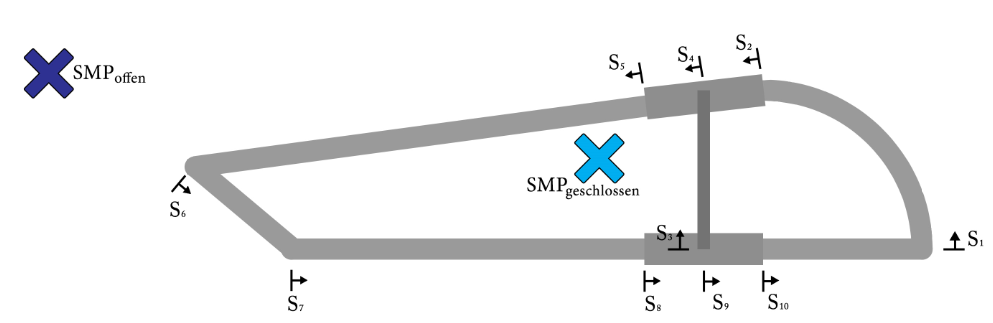
\includegraphics[width=1\textwidth]{Bilder/SMP}
	\caption{Schubmittelpunkt des geschlossenen und offenen Profils}
\end{figure}
\subsubsection{Torsion (O.S.)}
\begin{figure}[h]
	\centering
	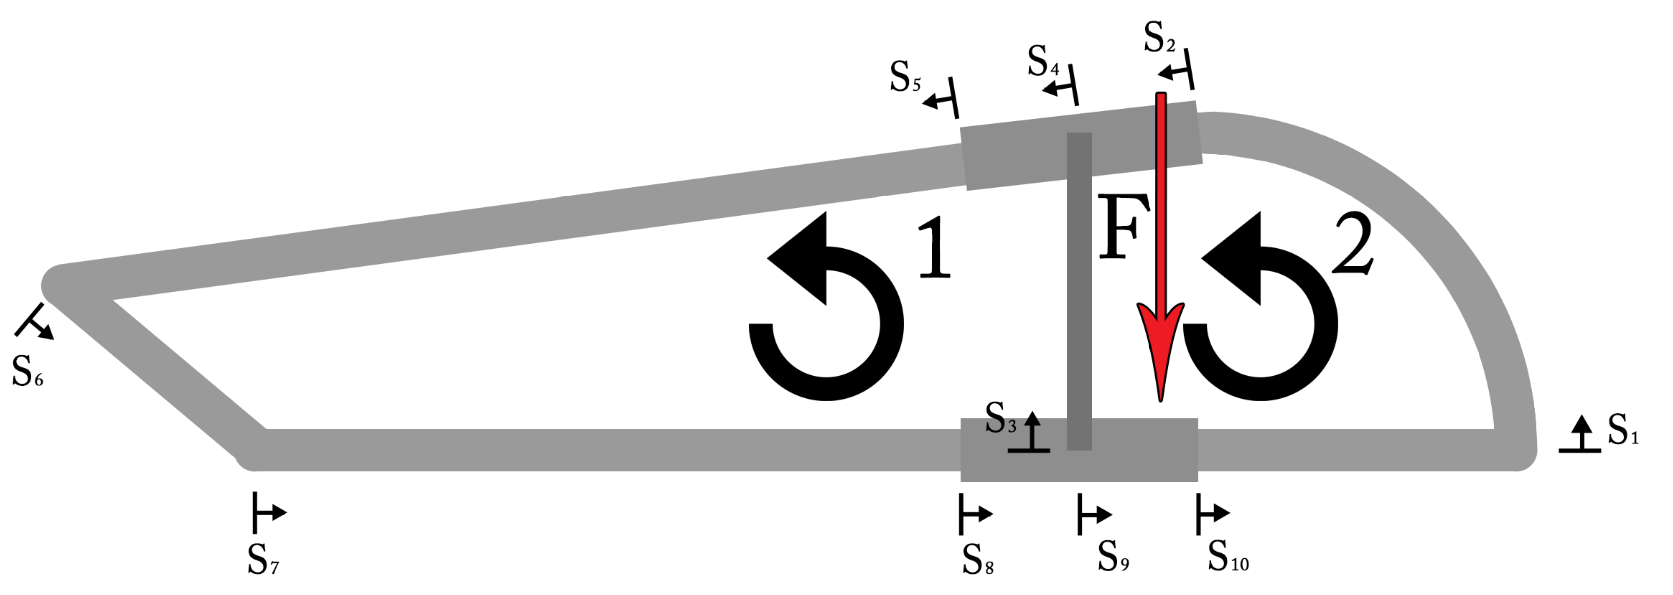
\includegraphics[width=1\textwidth]{Bilder/Torsion}
	\caption{Angreifende Kraft und positive Drehrichtung}
\end{figure}
In den bisherigen Berechnungen wurde immer davon ausgegangen, dass die Kraft im Schubmittelpunkt angreift. Durch den Versuchsaufbau ist jedoch vorgegeben, dass eine Prüflast in z-Richtung an den $l/4$-Linie aufgebracht wird. Mit dem errechneten Schubmittelpunkt lässt sich erkennen, dass ein Torsionsmoment 
\begin{equation}
	M_{xT}=(y_{l/4}-y_{0})\cdot F
\end{equation}
entsteht, das noch zusätzlichen Schubfluss und eine Verwindung $\vartheta$ bewirkt. Genauer gesagt wird hier die St. Vernatsche Torsion behandelt, bei der zwar Verwölbung auftritt, diese aber nicht behindert wird \cite{item15}. Wieder können die konstanten Schubanteile $q_{0T,i}$ aus der Momentenäquivalenz und der Verwindung bestimmt werden. Wobei zu beachten ist, dass die Verwindung hier nicht mehr wie bei der reinen Biegung null ist, aber über die Verträglichkeitsbedingung weiterhin gelten muss
\begin{equation}
	\vartheta_{1}=\vartheta_{2}=\vartheta.
\end{equation}
Da die bisherigen Anteile des Schubflusses definitionsgemäß weder Verwindung verursachen, noch bezüglich des Schubmittelpunkts ein Moment kompensieren, fallen sie aus den Gleichungen raus. Es bleiben nur noch die Konstanten $q_{0T,i}$ übrig. Damit ergeben sich die vereinfachten Formeln für die Verwindung und die Momentenäqivalenz:
\begin{equation}\label{verdrillung}
	\vartheta_{i} = \frac{1}{2A_{0i}G}(q_{0T,i}\oint\frac{1}{t(s)}ds-q_{0T,i\pm1}\int\frac{1}{t(s)}ds)
\end{equation}
\begin{equation}
		M_{xT}=2\sum q_{0T,i}\cdot A_{0i}
\end{equation}
Für eine maximale Prüflast von $F=500\mathrm{N}$ die der Flügel aushalten muss, erhält man
$$
	q_{0T,1}=-1,80\mathrm{N/mm}
$$
$$
	q_{0T,2}=-1,87\mathrm{N/mm}.
$$
Setzt man nun diese Werte in Gleichung (\ref{verdrillung}) erhält man für beide Zellen einer Verwindung von
$$
	\vartheta =-0,00242 ^\circ.
$$
Integriert man diesen konstanten Wert über die gesamte Länge des Flügels, erhält man den Drillwinkel am Ende mit $\varphi = -1,87^\circ$.

\subsubsection{Schubspannung (O.S.)}
Das Ziel dieser Berechnung war nicht nur den Schubmittelpunkt und den Drillinkel zu bestimmen, sondern hauptsächlich die Schubspannung in der Haut zu erhalten, um diese auslegen zu können. Da die Hautdicke auf dem gesamten Umfang konstant bleiben soll, ist an dieser Stelle nur die maximale Schubspannung für alle Bereiche der Haut $\tau_{max}$, die sich einfach aus Gleichung (\ref{tau}) ermitteln lässt, interessant. Die Dicke $t$ ist jedoch nicht einfach aus den gesamten Rechnungen rausziehbar, weil es auch Anteile, wie zum Beispiel den Holm, gibt, die von $t$ unabhängig sind. Deswegen wird iterativ vorgegangen, wobei zuerst mit einer zufällig gewählten Dicke die Rechenschritte durchgeführt werden, in dem in diesem Kapitel gezeigten Fall mit $t=0,2\mathrm{mm}$. Am Ende der Berechnung wird aus den maximalen Schubfluss die minimale Dicke
\begin{equation}
	t_{min} = \frac{q_{max}}{R_{\tau}}.
\end{equation} 
bestimmt. Die Festigkeit bei reiner Schubbelastung $R_{\tau} = 166,67\mathrm{N/mm^2}$ wurde mittels ELamX bestimmt. Diese Dicke kann jedoch nicht als einfach so als Ergebnis genommen werden, da sich der Schubfluss mit variabler Dicke mit verändert. Die Rechnung muss mit dem neuen Wert erneut durchgeführt werden. Somit nähert man sich Schritt für Schritt dem Idealwert, bei dem die vorliegende Dicke der minimalen Dicke entspricht.

Nach einigen Iterationen bildet sich der Wert $t = 0,03\mathrm{mm}$ als Grenzwert heraus. Da dies ungefähr 0,4 Lagen bei einer Dicke $0,0783\mathrm{mm}$ des $\pm45^\circ$-Gewebes entspricht, muss für die Fertigung des Flügels auf eine ganzzahlige Lagenanzahl aufgerundet werden. Hier wurde eine Dicke von 
\begin{equation}
	t = 0,1566 \mathrm{mm}
\end{equation}
gewählt, was $2$ Lagen entspricht. Dies macht einen symmetrischen Aufbau der Haut möglich und gewährleistet die beste Beulsteifigkeit. Außerdem ist eine ausreichende Sicherheit in Folge der getroffenen Vereinfachungen gewährleistet.

Mit dieser Dicke verändern sich die Werte des endgültigen Flügels im Vergleich zu den bisher in diesem Kapitel mit $t=0,2\mathrm{mm}$ durchgeführten Berechnungen. Der Schubmittelpunkt verschiebt sich minimal zu
$$
	y_{M_{g}}=75,72\mathrm{mm}
$$
$$
	z_{M_{g}}=-21,31\mathrm{mm}.
$$
Auch der Drillwinkel vergrößert sich leicht durch die gesenkte dünnere Haut Steifigkeit zu
$$
	\varphi =-2,32 ^\circ.
$$
Aus den Verläufen der Schubflüsse, wie sie in Abbildung \ref{fig:S1}-\ref{fig:S10} zu sehen, erkennt man, dass die betragsmäßig maximale Schubspannung am Endpunkt des Bereichs 8 auftritt.
$$
	|\tau_{max}|=\tau(s_8=14)=47,52\mathrm{N/mm^2}\leq R_{\tau}
$$
Im Steg (Bereich 3) tritt zwar ein deutlich höherer Schubfluss auf, jedoch ergibt sich durch die ebenfalls deutlich höhere Dicke eine geringere Spannung.







